\section{Approach}
\subsection{Overview}
\subsection{Motivation for Monte Carlo in Spark}
% Why Monte Carlo is a promising approach for memory-efficiency.
% \subsubsection{Limitations of Iterative PageRank}
% \subsubsection{Idea of Monte Carlo Random Walks}
% \subsubsection{Approximation vs. Convergence Trade-off}
% \subsubsection{Advantages in Spark Environments}

The Monte Carlo method is an alternative approach to the traditional PageRank implementation. Instead of iteratively computing the entire rank vector, it focuses on simulating random walks on the graph. In this approach, a specified number of walkers are released per node, and they then traverse the graph according to the "random surfer" model. Similar to the original algorithm, a random surfer follows an outgoing link with probability $\alpha$ or teleports to a random node in the graph with probability $1-\alpha$. Ultimately, the PageRank values are estimated by the relative frequency with which a node was visited by random walkers. The key difference from the iterative approach is that the walkers take a predefined number of steps instead of updating the rank vector until convergence. Thus, the Monte Carlo approach can control memory usage by limiting the number of walkers and steps, making it a promising candidate for approximating the PageRank of large-scale graphs \cite{avrachenkov_monte_2007}. \par
Additionally, estimating PageRank values is sufficient for many applications. For real-world tasks such as website ranking or user recommendation on social networks, the only things of interest are a node's relative importance and the stability of the ranking. Therefore, total convergence of the PageRank vector is unnecessary. The approximate Monte Carlo approach achieves significant memory and computational savings with only a slight loss in accuracy. This balance between performance and accuracy enables graph analytics on graphs that would otherwise be too large to handle.\par
Furthermore, implementing Monte Carlo PageRank in a Spark environment utilizes a distributed data processing framework that includes Spark's Resilient Distributed \allowbreak Datasets (RDDs). This data structure can represent the entire graph and the walker's state at every step. Spark's properties, such as fault tolerance through lineage and efficient in-memory computation, make it a more attractive platform than the iterative PageRank method for evaluating the Monte Carlo PageRank method. Of particular interest is whether the Monte Carlo approach can operate under limited memory conditions while achieving sufficient accuracy and maintaining low variance throughout the ranking. \par
This thesis explores the integration of such an approximate Monte Carlo method in the Spark environment and evaluates it's performance and accuracy on limited memory usage in comparison to the standard GraphX PageRank method.
 

\subsection{Algorithm Design}
% Describe how RDDs are used for graph and walker states.

% \subsubsection{Initialization of Walkers}
% \subsubsection{Step-by-Step Simulation Process}
% \subsubsection{Random Number Generation and Reproducibility}
% \subsubsection{Handling Dangling Nodes}
% \subsubsection{Computation of Approximate PageRank Scores}

The approximate Monte Carlo algorithm estimates the stationary distribution by leveraging a step by step simulation that follows the random surfer model.
The pseudo code bellow presents the walker simulation and the decision logic used in each step.

\vspace{1.5em}
\begin{algorithm}[H]
\caption{Monte Carlo PageRank Approximation}
\KwIn{Graph $G=(V,E)$, walkers per node $w$, number of steps $k$, damping factor $\alpha$}
\KwOut{Approximate PageRank scores $\hat{\pi}(v)$ for all $v \in V$}

\ForEach{node $v \in V$}{
Initialize $w$ walkers at $v$
}
\For{step = 1 to $k$}{
\ForEach{walker $i$ at node $u$}{
Generate random number $r \in [0,1]$;
\eIf{$r < \alpha$ \textbf{and} $u$ has outgoing edges}{
Move walker to a random neighbor of $u$;
}{
Teleport walker to a random node $v \in V$;
}
}
}
\ForEach{node $v \in V$}{
$\hat{\pi}(v) \gets \frac{\text{Number of walkers at } v}{|V| \cdot w}$
}
\end{algorithm}
\vspace{1.5em}

The algorithm initializes $w$ walkers per node, which is resulting in a total number of $w\cdot |V|$ walkers. Each walker is randomly distributed throughout the graph. Then, each walker simultaneously performs a number of $k$ independent steps.
At each step, the walker $w$ generates a random number between $0$ and $1$. To ensure deterministic behavior, each walker uses a seeded random number generator that guarantees reproducibility:

\vspace{0.5em}
\newpage
\begin{lstlisting}[caption={Materializing and Unpersisting Walker RDD},
                   label={lst:walker},
                   captionpos=b] 
val seed = System.nanoTime + Thread.currentThread().getId + step + currentNode.toInt
\end{lstlisting}


\vspace{0.5em}

In case a node does not have any outedges, it's treated as a dangling node and the walker will directly teleport to a random node.
After $k$ steps the simulation terminates and the PageRank values are approximated based on the walker visits of a node.

\subsection{Implementation in Spark}
% \subsubsection{Graph Representation with RDDs}
% \subsubsection{Adjacency List Construction}
% \subsubsection{Broadcasting for Teleportation}
% \subsubsection{Walker State Representation and Distribution}
% \subsubsection{RDD Caching, Materialization, and Unpersisting}
% \subsubsection{Repartitioning for Load Balancing}

The Monte Carlo Implementation is structured around two main components: The graph representation and the walker states. Both of them are stored in Sparks RDDs, which make them suitable for processing in a distributed system.

At the beginning of the program a given edge list file is read to get the structure of the graph. It is stored as an RDD of directed edges. Then by grouping the outgoing neighbors of each node an adjacency list is constructed, which is one of the main RDD-based components, that is represnting the entire graph structure:

\vspace{0.5em}
\begin{lstlisting}[language=Scala, caption={Adjacency list creation}, label={lst:adjlist}]
val adjList: RDD[(Long, Iterable[Long])] = edgesRDD.groupByKey().cache()
\end{lstlisting}
\vspace{0.5em}

Additionally, an array of all vertices is required to support teleportation. This list will be distributed as a broadcasting variable to all nodes.

\vspace{0.5em}
\begin{lstlisting}[language=Scala, caption={Broadcasting Variable}, label={lst:broadcast}]
val broadcastNodes = sc.broadcast(allNodesArray)
\end{lstlisting}
\vspace{0.5em}

This mitigates costly network shuffles during every teleportation. Because the set of nodes is required in every simulation step it is cached in memory for efficient access.
A fixed number of walkers are initialized and represented in a seperate RDD. The RDD is distributed across multiple partitions to ensure efficient parallel processing and scaling when analyzing large graphs. Each entry in the RDD is a random vertex ID, representing the current vertex of a walker. In each simulation step the walker RDD is joined with the adjacency list to get all possible outgoing edges. After each walker updates its position, a new walker RDD is initialized with the updated positions. Before the previous walker RDD is explicitly unpersisted after the step is completed, the new walker RDD has to be materialized.
\newpage
\begin{lstlisting}[language=Scala, caption={Materializing and Unpersisting Walker RDD}, label={lst:materialize}]
nextWalkersRDD.cache() 
nextWalkersRDD.count() // trigger an action to materialze RDD
walkersRDD.unpersist(blocking = false)
\end{lstlisting}
\vspace{0.5em}
This is because Spark uses lazy evaluation. It ensures that only the current walker RDD and the adjacency list occupy memory. \par
Before caching the walkers RDD in memory, repartitioning is applied to the RDD after each step. This is crucial for balanced distribution across partitions as it ensures that the number of partitions remains the same throughout the experiment. 
When processing large graphs that include nodes with high ingoing edges it prevents skews and stragglers allowing Spark to efficiently use all available cores. Managing the partitions correctly can have a significant impact on performance. 


\subsection{Experimental Framework and Automation}

% \subsubsection{Datasets: Real-World and Synthetic Graphs}
% \subsubsection{Synthetic Graph Generation}
% \subsubsection{Parameter Variation in Experiments}
% \subsubsection{Spark Cluster Setup}
% \subsubsection{Automation via Shell Scripts}
% \subsubsection{Data Collection and Visualization}

Finally, to evaluate the performance of the approximate Monte Carlo method an experimental framework was established, that aims for reproducibility. It benchmarks the Monte Carlo method and compares it to the standard PageRank method. The evaluation is focusing mainly on memory efficiency while trading off performance and accuracy. \par
The datasets used for evaluation include both real-world and synthetic graphs. Real-world graphs such as wiki-Talk provide an irregular graph structure and millions of edges, presenting a practical use case. On the other hand, synthetic graphs of any size and with different characteristics can be generated. In the experiments, Erdős–Rényi graphs of different sizes, ranging from $100.000$ to $20$ million nodes, have been generated. To establish comparable conditions between the different graph sizes, the density is kept consistent by controlling the number of outgoing edges per node. However, the in-degree of each node is random and ranges between $0$ and $n-1$, where $n$ is the total number of nodes. A simple python script is used to generate and store the graph structure in an edge list file.

\vspace{1.5em}
\begin{algorithm}[H]
\caption{Synthetic Graph Generator}
\KwIn{Range of node counts $[N_{\min}, N_{\max}]$, step size $\Delta N$, edges per node $E$}
\KwOut{Synthetic graph files with $E$ outgoing edges per node}

Set random seed for reproducibility\;
\For{$n \gets N_{\min}$ \KwTo $N_{\max}$ \KwStep $\Delta N$}{
  Create output file for graph with $n$ nodes\;
  \ForEach{node $u \in \{1, \dots, n\}$}{
    \For{$i \gets 1$ \KwTo $E$}{
      Select random destination $v \in \{1, \dots, n\}$\;
      \If{$v \neq u$}{
        Write edge $(u, v)$ to file\;
      }
    }
  }
  
}
\end{algorithm} 
\vspace{1.5em}

The output can be directly used for Spark processing.\par
During the experiments, the main parameters of the Monte Carlo method have been varied. The parameters include the number of walkers and the number of steps per walker. The goal was to systematically compare performance, memory and runtime across varying parameters. In the GraphX implementation the only parameters that were configured are the tolerance and the damping factor. The tolerance is usually set to $0.001$. In the experiments it was kept on such a low value to get very precise PageRank values and to compare the approximate Monte Carlo approach to the standard PageRank method. The reset probability was set to $0.15$ for both methods. Additionally, different Spark configurations were analyzed such as the number of executors and most importantly the memory allocated per executor. \par



To automate the experiments, shell scripts are used. Each script relies on spark-submit, which is the standard command line tool used to launch applications on a Spark cluster. In the spark-submit command configurations such as the number of executors and the memory per executor can be set. Furthermore, the edge list file is passed to the script as well as the Monte Carlo specific configuration such as the number of walkers and steps per walker. This setup ensures that experiments are running in a sequence without needing manual input and with consistency throughout multiple data sets. Finally, the spark-submit command allows to either run the applications locally or to launch them to a cluster environment to simulate a real distributed system. \par

To ensure comparable conditions across all experiments, all experiments are executed on a Spark cluster set up on the university's server. For simplicity, the Spark cluster is deployed in standalone mode, which is a built-in cluster manager. Only the master and workers need to be started on the university server. The cluster consists of one master node and four worker nodes. Each worker node has one executor with two cores, for a total of eight cores. \par


In every experiment, metrics for both methods are collected, including configurations such as the number of walkers and steps for the Monte Carlo method. Another file collects the total runtime, allocated memory, and graph size to evaluate performance with limited memory and with different graph sizes. For accuracy evaluation, the top 20 ranks for both methods are saved in a separate file. \par
All the collected data is saved in CSV files to efficiently analyze it in the next step. With the help of Python scripts and the use of libraries such as Matplotlib and Pandas, the data is structured and visualized in various plots of runtime, allocated memory, accuracy and cost. This provides a clear overview of the data and enables a thorough analysis of the data. \par
This setup ensures the reproducibility and scalability of evaluating the Monte Carlo method. This is achieved through the use of various datasets, such as real-world and synthetic data, as well as a systematic variation in parameters. Additionally, scripts automate experiments and efficiently collect key metrics. This framework enables the analysis of the empirical results presented in the following sections. \par
\begin{figure}[H]
    \centering
    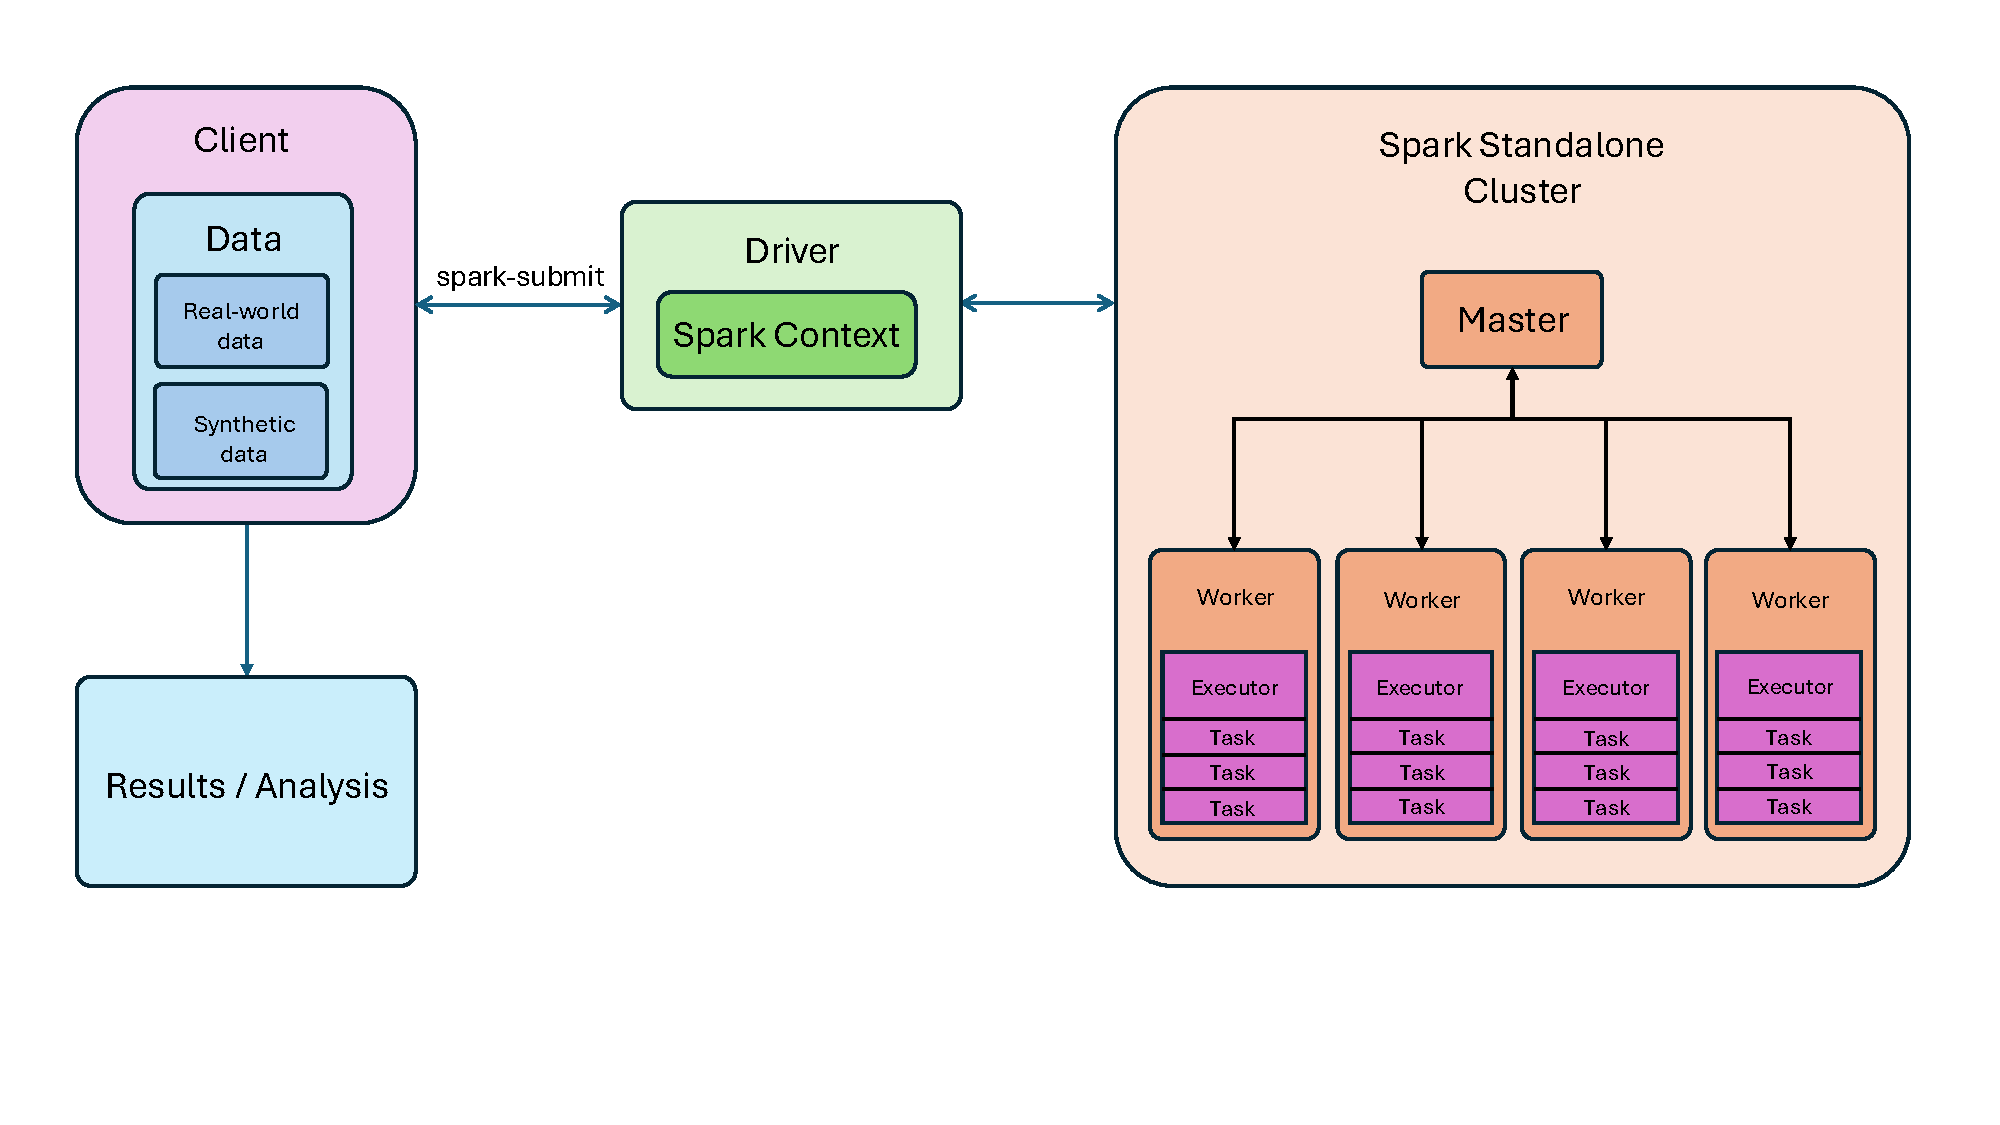
\includegraphics[width=\linewidth]{images/Workflow_image.pdf}
    \caption{Experimental Workflow}
    \label{fig:workflow}
\end{figure}
Finally, the given approach combines an approximate Monte Carlo implementation with a distributed Spark environment and a systematic experimental framework. The main goal of this setup is to determine whether the described method can operate with much less memory than the standard PageRank implementation. While a trade-off in accuracy and performance is expected and tolerated, the method aims to provide sufficient accuracy and performance. The evaluation will reveal whether the Monte Carlo approach is a viable alternative to the standard PageRank method in environments with restricted memory and large-scale graphs, addressing the central research question of this thesis.


\subsection{Error Handling}
% \subsubsection{Out-of-Memory Handling}
% \subsubsection{Crash Scenarios Encountered During Experiments}
% \subsubsection{Timeout: How and when to cancel an Experiment}

When processing large-scale graphs, memory exhaustion and application crashes are inevitable. Therefore, error-handling strategies are necessary to ensure that experiments remain reproducible and manageable. For simplicity, this thesis only differentiates between out-of-memory (OOM) failures and timeouts. \par
The Java Out-of-Memory exception is a common scenario that is expected in this experimental setup because the goal is to deliberately strain memory. This exception is usually thrown when there is not enough memory in the Java heap to allocate to an object. This means the garbage collector is unable to free up enough space for the object. In these experiments, the exception was detected in the log files. In that case, the configurations are automatically marked as failed and excluded from further experiments. \par
Since very large graphs are being processed, some experiments can take a disproportionately long time to finish. This is why a timeout mechanism is implemented to prevent experiments from blocking the pipeline. If an experiment does not finish within the predefined time, the current experiment is terminated, and the next experiment with different configurations begins. This ensures that all experiments finish within an acceptable time frame.  \par
These error handling strategies establish a more systematic and stable process. Experiments can run without manual intervention, and the resulting datasets are more consistent.

